\subsection{Context: Mobile Crowd-Sensing Platforms}





Users may not want to contribute in a sensing system if their privacy is engage.

Crowd-sensing platforms are systems that collect and aggregate knowledge from a large amount of devices.
APISENSE is one of these platform that provide to scientists an easy way to deploy their sensing experiments in the wild. By using these platforms they can test their theories on real data instead of simulated one.



These data come from users that subscribe to data collect campaign and contribute with their mobile devices.





The data anonymization is mad on the server side.

With this approach we must trust the centralized server.


Crowd-sensing platforms have a large application domain.
Applications encompass application performance monitoring (\emph{e.g.}, OpenSignal\footnote{\url{http://opensignal.com}}), environment monitoring (air quality\footnote{\url{http://citizensensor.cc}}), etc.


Currently, the system uses a centralized approach where each smartphone individually report data to a central server.

Datasets are anonymized \emph{a posteriori}~\cite{DBLP:conf/icdcs/PrimaultMB15}, which does not protect from malicious behaviors during the upload phase.

\subsection{Motivations: Data Dissemination Threats}

A key challenge in the crowd-sensing platforms is to avoid central trusted server that present a single point of failure that need to be address.

Let imagine a user named Alice that participate to a data collect campaign.
Alice produces data and sends it directly to the central server.
In this scenario the server knows that Alice is the producer of the data that she sends.

Even if we have a strong trust in the central server about keeping users' data safe, this server is a target of choice for an attacker.
The security of the server can be compromized and users data can be stollen in a single attack on the server.
This kind of architecture is not safe because of its single rupture point.

Moreover, in the case of APISENSE architecture, collect servers can be maintain by other organizations that could keep informations about users before sending their data to the trusted central server.
This kind of treats is not acceptable in a privacy way.

To address this scenario, we think-off a method where user 

\begin{figure*}[t]
	\centering
	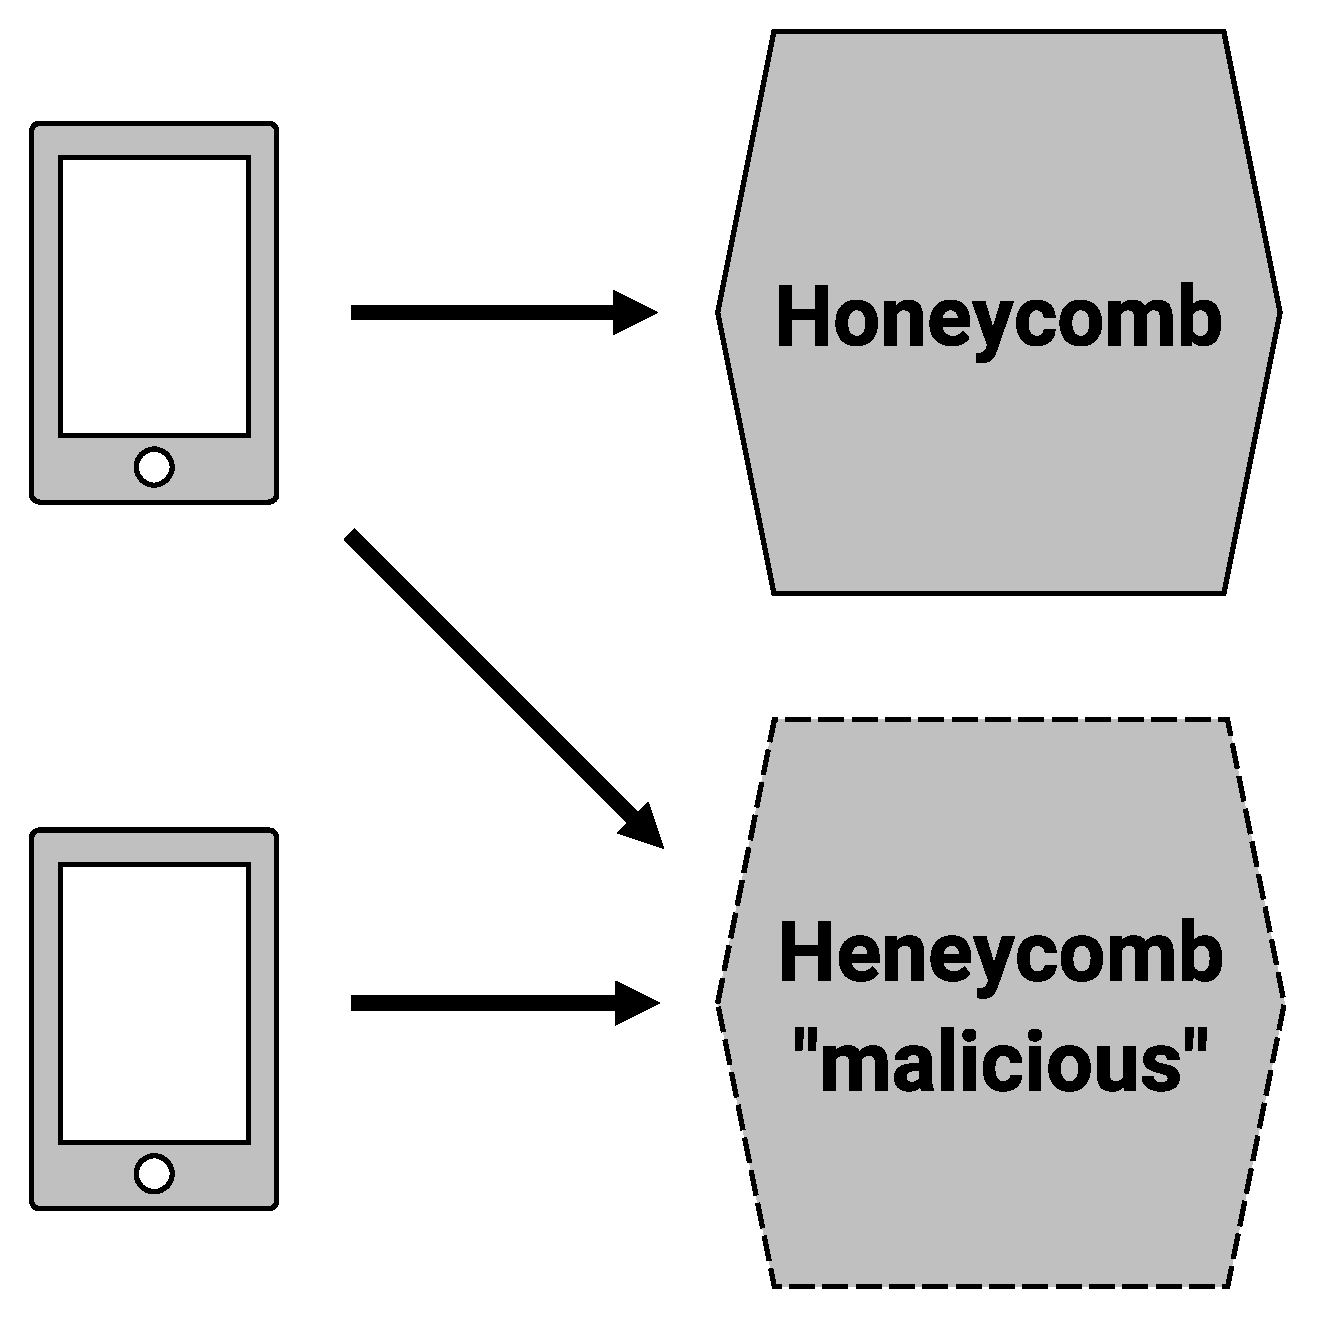
\includegraphics[width=0.4\textwidth]{figures/honeycomb}
	\caption{\label{Honeycomb} APISENSE data collection treat}
\end{figure*}

\subsection{Goals: Enabling Decentralized Dissemination}

Our approach uses too delay tolerant networks because we do not care about what time a data makes to be sended to the server. We want privacy first.

Our objective is to trend to \emph{Privacy-by-Design}~\cite{langheinrich2001privacy} principles by making a decentralized dissemination without compromising the quality and the utility of the collected data.
